%% arrowLength=10
%% linkWidth=3
%% input fy=50*node.pos
%% output fx=350
%% output fy=50*node.pos+50
%% MAX_FONT_SIZE=8
\begin{table}[H]
    \begin{center}
        \begin{tabular}{||l c c c||}
            \hline
            & 1        & 2        & 3 \\ [0.5ex]
            \hline
            velikost populacije               & 200      & 250      & 350      \\
            \hline
            največje število globokih vozlišč & 15       & 20       & 40       \\
            \hline
            največje število povezav          & 30       & 50       & 100      \\
            \hline
            največje število prečkanj         & 2        & 3        & 4        \\
            \hline
            delež mutiranih potomcev          & 10\%     & 10\%     & 10\%     \\
            \hline
            prispevek kompleksnosti           & -0.00001 & -0.00001 & -0.00001 \\
            \hline
            število generacij                 & 200      & 200      & 300      \\
            \hline
        \end{tabular}
    \end{center}
    \caption{Nabori inicializacijskih parametrov poganjanja na množici Car Evaluation.}
    \label{tab:param_car}
\end{table}

\subsection{Prvi nabor}\label{subsec:dodatek-car-prvi-nabor}
%%"/home/jure/CLionProjects/Neuroevolution/datasets/car/car.data" 200 15 30 2 true 0.1 100 true -0.00001 200 ACC
\begin{table}[H]
    \begin{center}
        \begin{tabular}{|| c | c c || c c ||}
            \hline
            \multirow{2}{*}{št. zagona} & \multicolumn{2}{c||}{točnost najboljšega agenta} & \multicolumn{2}{c||}{MCC najboljšega agenta} \\ \cline{2-5}
            & učna   & testna          & učna  & testna                  \\
            \hline
            1        & 72.1\% & 69.5\%          & 0.469 & \textbf{0.530 (71.8\%)} \\
            \hline
            2        & 73.1\% & 70.8\%          & 0.473 & 0.504                   \\
            \hline
            3        & 71.6\% & 70.5\%          & 0.470 & 0.400                   \\
            \hline
            4        & 71.8\% & \textbf{72.2\%} & 0.484 & 0.446                   \\
            \hline
            5        & 71.5\% & 71.0\%          & 0.478 & 0.463                   \\
            \hline
            $\sigma$ & 0.006  & 0.009           & 0.006 & 0.045                   \\
            \hline
        \end{tabular}
    \end{center}
    \caption{Rezultat prvega nabora parametrov.}
    \label{tab:car_result_1}
\end{table}

\begin{table}[H]
    \centering
    \begin{tabular}{||rccccc||}
        \hline
        razred       & unacceptable & acceptable & good & very good & vsota \\ \hline
        unacceptable & 363          & 0          & 0    & 0         & 363   \\ \hline
        acceptable   & 111          & 0          & 0    & 4         & 115   \\ \hline
        good         & 21           & 0          & 0    & 0         & 21    \\ \hline
        very good    & 0            & 0          & 0    & 11        & 19    \\ \hline
        vsota        & 503          & 0          & 0    & 15        & 518   \\ \hline
    \end{tabular}
    \caption{Matrika zmot najbolj točnega agenta prvega nabora. Agent lahko napove samo razreda \enquote{nesprejemljivo} in \enquote{zelo dobro}.}
    \label{tab:car_acc_1}
\end{table}

\begin{table}[H]
    \centering
    \begin{tabular}{||rccccc||}
        \hline
        razred       & unacceptable & acceptable & good & very good & vsota \\ \hline
        unacceptable & 260          & 103        & 0    & 0         & 363   \\ \hline
        acceptable   & 3            & 112        & 0    & 0         & 115   \\ \hline
        good         & 0            & 21         & 0    & 0         & 21    \\ \hline
        very good    & 0            & 19         & 0    & 0         & 19    \\ \hline
        vsota        & 263          & 255        & 0    & 0         & 518   \\ \hline
    \end{tabular}
    \caption{Matrika zmot agenta z največjim MCC prvega nabora. Agent lahko napove samo razreda \enquote{nesprejemljivo} in \enquote{sprejemljivo}.}
    \label{tab:car_mcc_1}
\end{table}

\begin{figure}[H]
    \begin{center}
        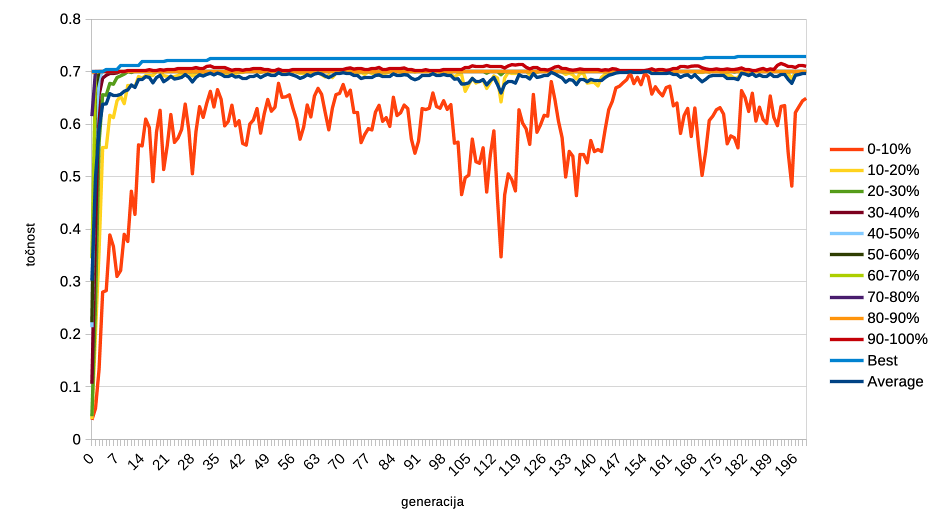
\includegraphics[width=13cm]{car/1/acc}
    \end{center}
    \caption{Graf točnosti populacije najboljšega agenta prvega nabora skozi generacije.}
    \label{fig:car_acc_1}
\end{figure}

\begin{figure}[H]
    \begin{center}
        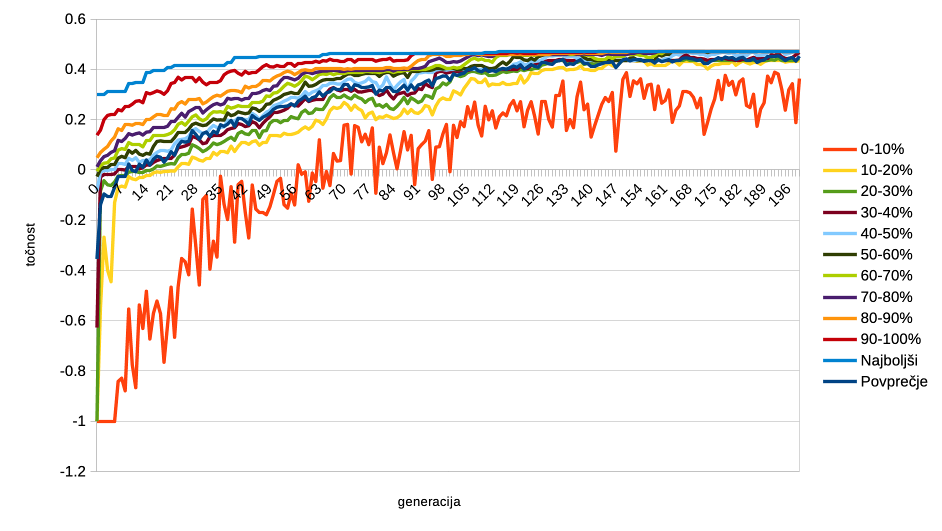
\includegraphics[width=13cm]{car/1/mcc}
    \end{center}
    \caption{Graf MCC populacije najboljšega agenta prvega nabora skozi generacije.}
    \label{fig:car_mcc_1}
\end{figure}

\begin{figure}[H]
    \begin{center}
        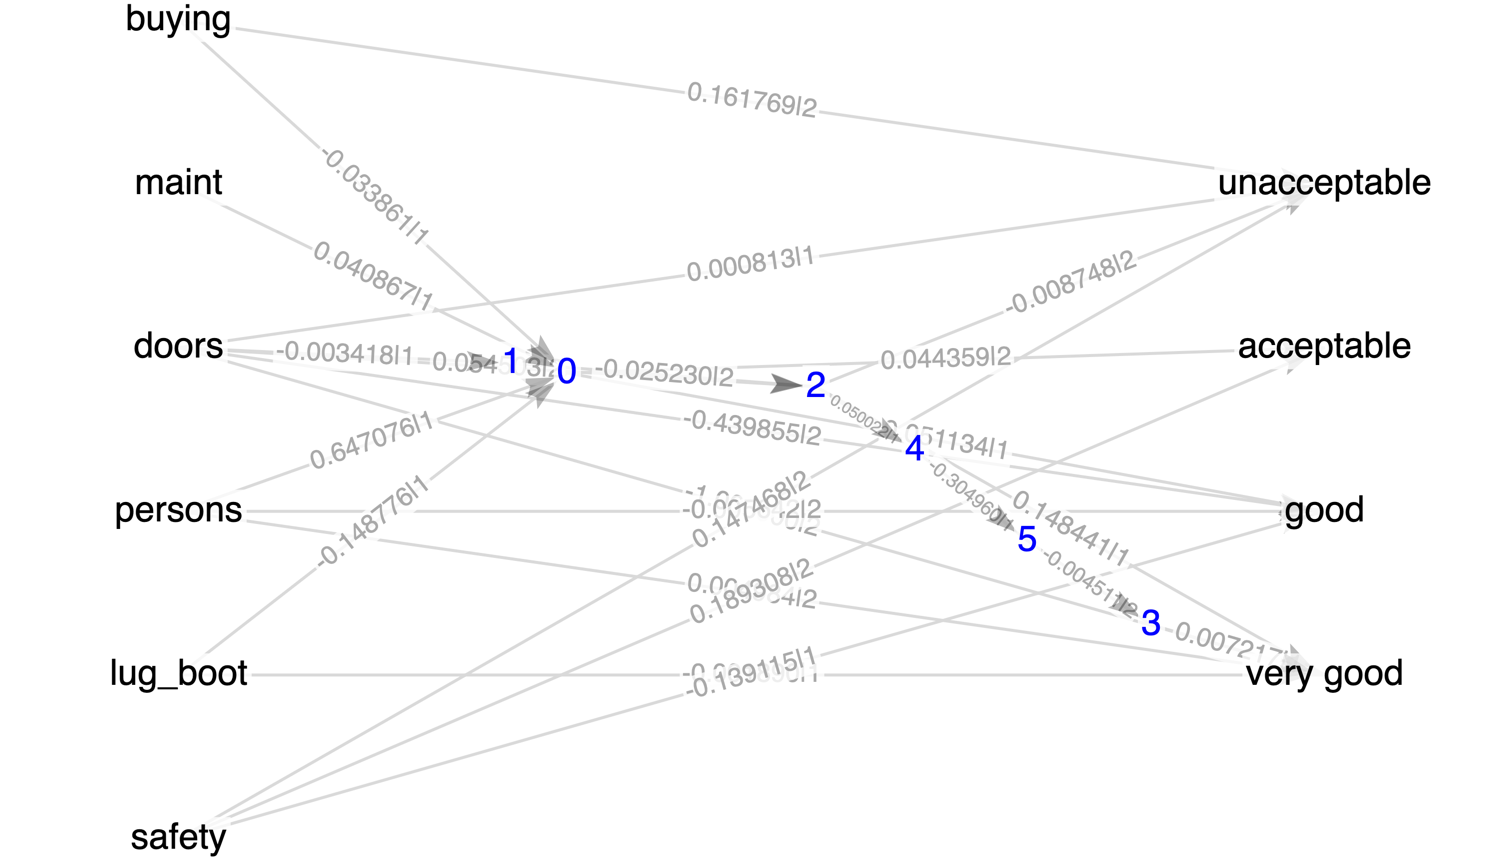
\includegraphics[width=13cm]{car/1/acc_g}
    \end{center}
    \caption{Vizualizacija najbolj točnega agenta prvega nabora. Vsebuje 7 povezav.}
    \label{fig:car_acc_1_g}
\end{figure}

\begin{figure}[H]
    \begin{center}
        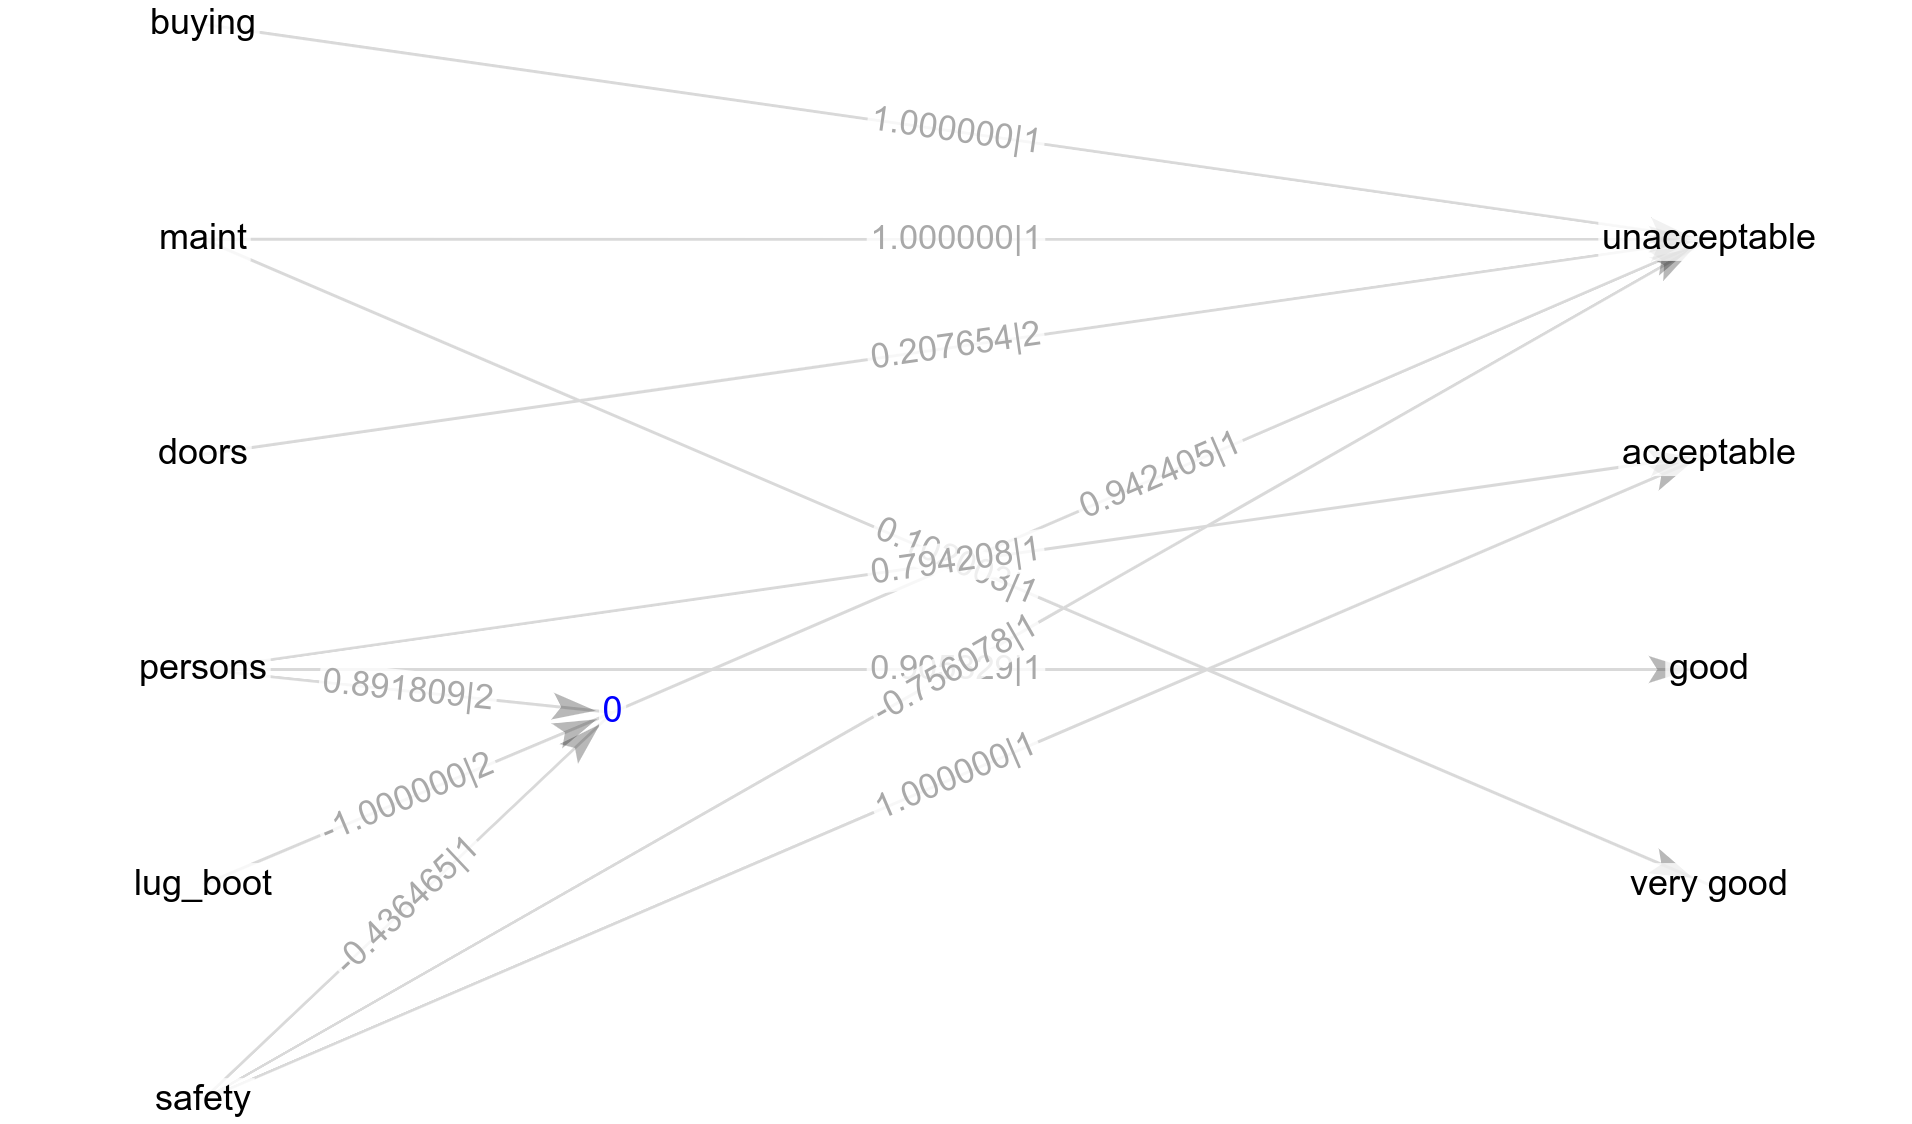
\includegraphics[width=13cm]{car/1/mcc_g}
    \end{center}
    \caption{Vizualizacija agenta z največjim MCC prvega nabora. Vsebuje 6 povezav.}
    \label{fig:car_mcc_1_g}
\end{figure}

\subsection{Drugi nabor}\label{subsec:dodatek-car-drugi-nabor}
%% 250 20 50 3 true 0.1 125 true -0.00001 200 ACC
\begin{table}[H]
    \begin{center}
        \begin{tabular}{|| c | c c || c c ||}
            \hline
            \multirow{2}{*}{št. zagona} & \multicolumn{2}{c||}{točnost najboljšega agenta} & \multicolumn{2}{c||}{MCC najboljšega agenta} \\ \cline{2-5}
            & učna   & testna          & učna  & testna                  \\
            \hline
            1        & 72.5\% & \textbf{74.3\%} & 0.480 & 0.419                   \\
            \hline
            2        & 71.1\% & 71.6\%          & 0.494 & 0.490                   \\
            \hline
            3        & 72.1\% & 71.8\%          & 0.481 & \textbf{0.514 (74.3\%)} \\
            \hline
            4        & 71.6\% & 71.0\%          & 0.483 & 0.454                   \\
            \hline
            5        & 74.4\% & 72.2\%          & 0.495 & 0.452                   \\
            \hline
            $\sigma$ & 0.011  & 0.011           & 0.007 & 0.033                   \\
            \hline
        \end{tabular}
    \end{center}
    \caption{Rezultat drugega nabora parametrov.}
    \label{tab:car_result_2}
\end{table}

\begin{table}[H]
    \centering
    \begin{tabular}{||rccccc||}
        \hline
        razred       & unacceptable & acceptable & good & very good & vsota \\ \hline
        unacceptable & 360          & 3          & 0    & 0         & 363   \\ \hline
        acceptable   & 90           & 25         & 0    & 0         & 115   \\ \hline
        good         & 10           & 11         & 0    & 0         & 21    \\ \hline
        very good    & 13           & 6          & 0    & 0         & 19    \\ \hline
        vsota        & 473          & 45         & 0    & 0         & 518   \\ \hline
    \end{tabular}
    \caption{Matrika zmot najbolj točnega agenta drugega nabora. Agent lahko napove samo razreda \enquote{nesprejemljivo} in \enquote{sprejemljivo}.}
    \label{tab:car_acc_2}
\end{table}

\begin{table}[H]
    \centering
    \begin{tabular}{||rccccc||}
        \hline
        razred       & unacceptable & acceptable & good & very good & vsota \\ \hline
        unacceptable & 286          & 77         & 0    & 0         & 363   \\ \hline
        acceptable   & 16           & 99         & 0    & 0         & 115   \\ \hline
        good         & 0            & 21         & 0    & 0         & 21    \\ \hline
        very good    & 0            & 19         & 0    & 0         & 19    \\ \hline
        vsota        & 302          & 216        & 0    & 0         & 518   \\ \hline
    \end{tabular}
    \caption{Matrika zmot agenta z največjim MCC drugega nabora. Agent lahko napove samo razreda \enquote{nesprejemljivo} in \enquote{sprejemljivo}.}
    \label{tab:car_mcc_2}
\end{table}

\begin{figure}[H]
    \begin{center}
        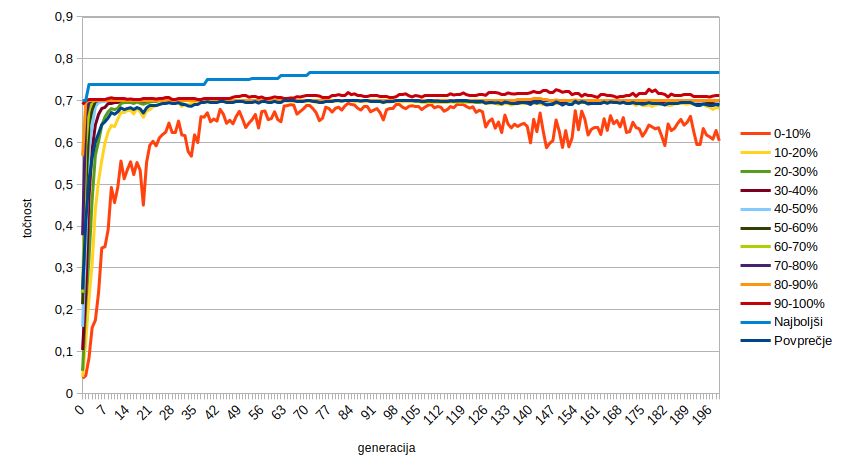
\includegraphics[width=13cm]{car/2/acc}
    \end{center}
    \caption{Graf točnosti populacije najboljšega agenta drugega nabora skozi generacije.}
    \label{fig:car_acc_2}
\end{figure}

\begin{figure}[H]
    \begin{center}
        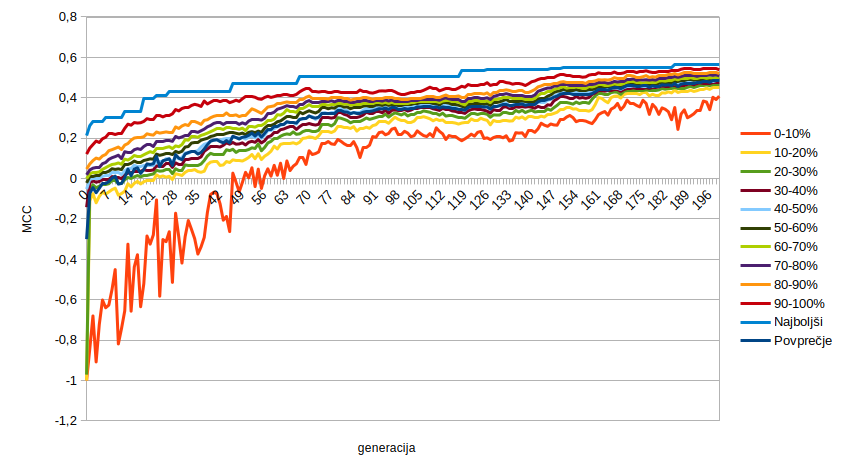
\includegraphics[width=13cm]{car/2/mcc}
    \end{center}
    \caption{Graf MCC populacije najboljšega agenta drugega nabora skozi generacije.}
    \label{fig:car_mcc_2}
\end{figure}

\begin{figure}[H]
    \begin{center}
        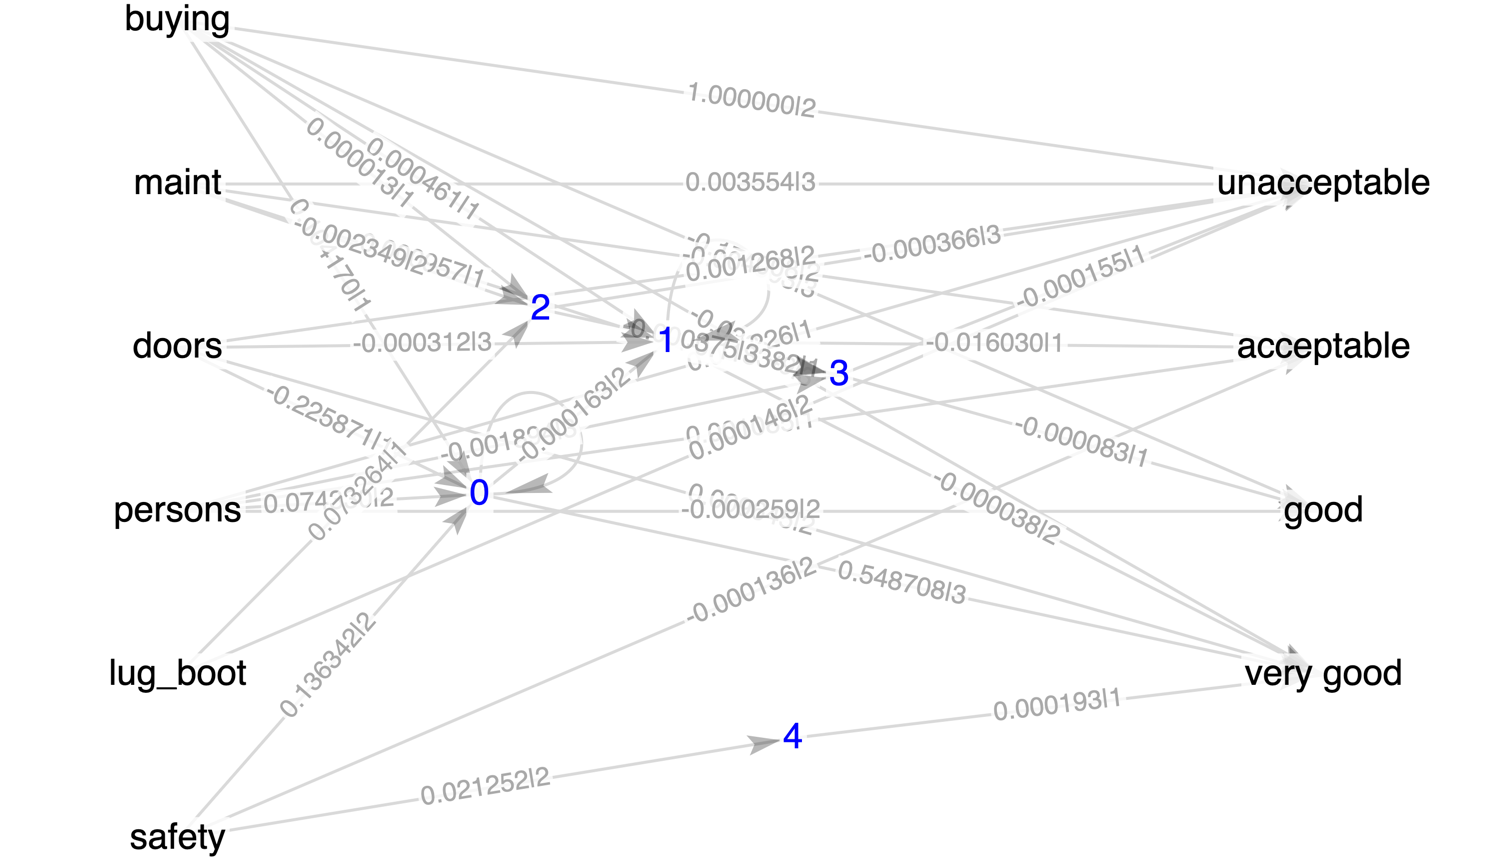
\includegraphics[width=13cm]{car/2/acc_g}
    \end{center}
    \caption{Vizualizacija najbolj točnega agenta drugega nabora. Vsebuje 8 povezav.}
    \label{fig:car_acc_2_g}
\end{figure}

\begin{figure}[H]
    \begin{center}
        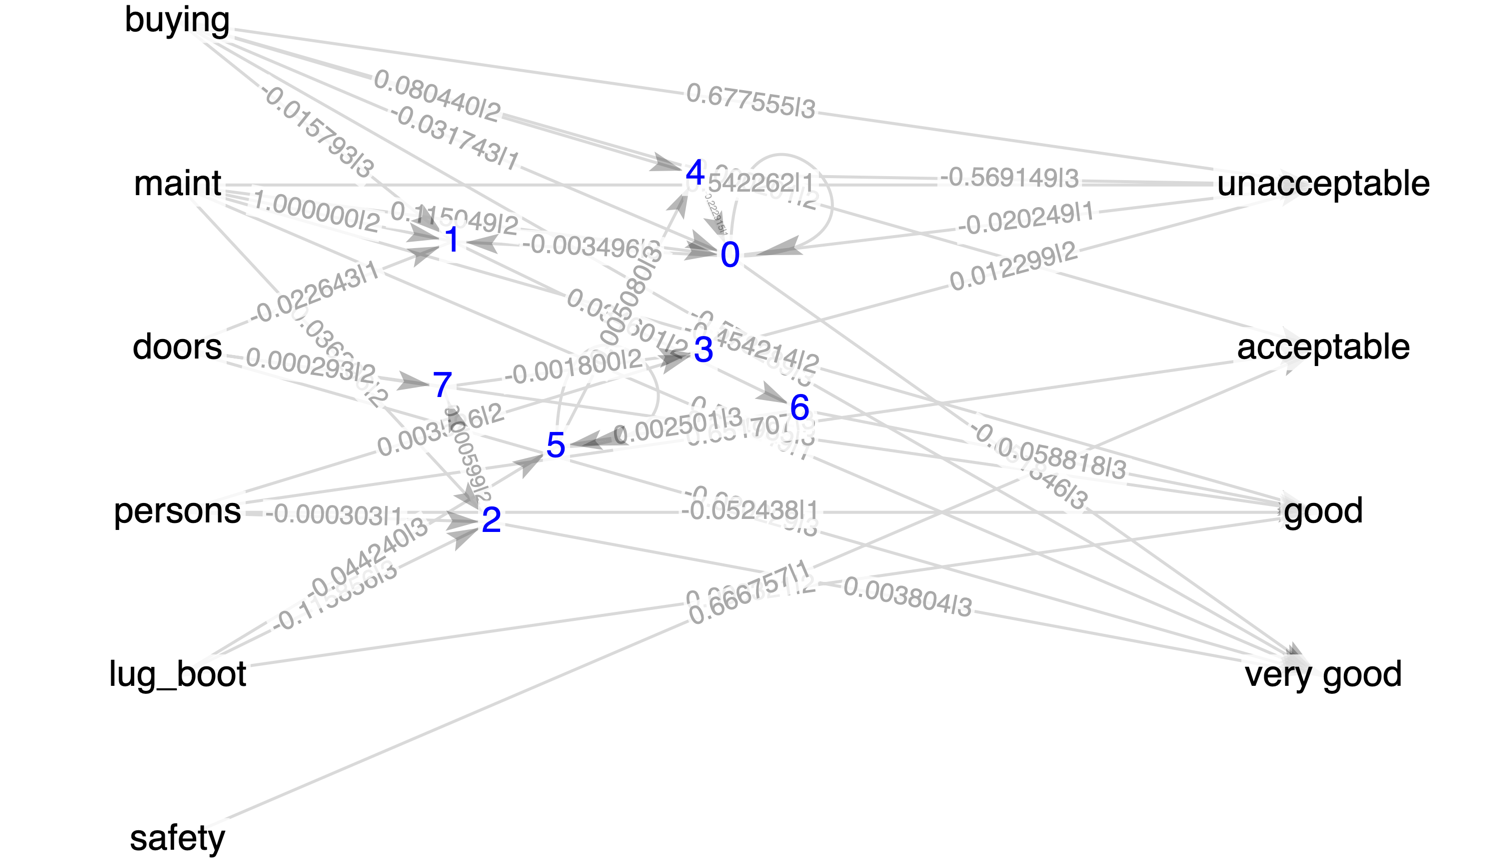
\includegraphics[width=13cm]{car/2/mcc_g}
    \end{center}
    \caption{Vizualizacija agenta z največjim MCC drugega nabora. Vsebuje 9 povezav.}
    \label{fig:car_mcc_2_g}
\end{figure}

\subsection{Tretji nabor}\label{subsec:dodatek-car-tretji-nabor}
%% 350 40 100 4 true 0.1 175 true -0.00001 300 ACC
\begin{table}[H]
    \begin{center}
        \begin{tabular}{|| c | c c || c c ||}
            \hline
            \multirow{2}{*}{št. zagona} & \multicolumn{2}{c||}{točnost najboljšega agenta} & \multicolumn{2}{c||}{MCC najboljšega agenta} \\ \cline{2-5}
            & učna   & testna          & učna  & testna                  \\
            \hline
            1        & 72.8\% & 72.6\%          & 0.496 & 0.447                   \\
            \hline
            2        & 72.9\% & \textbf{73.7\%} & 0.490 & 0.494                   \\
            \hline
            3        & 71.2\% & 70.7\%          & 0.495 & 0.477                   \\
            \hline
            4        & 71.1\% & 71.0\%          & 0.483 & 0.488                   \\
            \hline
            5        & 73.1\% & 73.2\%          & 0.488 & \textbf{0.520 (71.6\%)} \\
            \hline
            $\sigma$ & 0.009  & 0.012           & 0.005 & 0.024                   \\
            \hline
        \end{tabular}
    \end{center}
    \caption{Rezultat tretjega nabora parametrov.}
    \label{tab:car_result_3}
\end{table}

\begin{table}[H]
    \centering
    \begin{tabular}{||rccccc||}
        \hline
        razred       & unacceptable & acceptable & good & very good & vsota \\ \hline
        unacceptable & 340          & 23         & 0    & 0         & 363   \\ \hline
        acceptable   & 73           & 42         & 0    & 0         & 115   \\ \hline
        good         & 0            & 21         & 0    & 0         & 21    \\ \hline
        very good    & 0            & 19         & 0    & 0         & 19    \\ \hline
        vsota        & 413          & 105        & 0    & 0         & 518   \\ \hline
    \end{tabular}
    \caption{Matrika zmot najbolj točnega agenta tretjega nabora. Agent lahko napove samo razreda \enquote{nesprejemljivo} in \enquote{sprejemljivo}.}
    \label{tab:car_acc_3}
\end{table}

\begin{table}[H]
    \centering
    \begin{tabular}{||rccccc||}
        \hline
        razred       & unacceptable & acceptable & good & very good & vsota \\ \hline
        unacceptable & 261          & 102        & 0    & 0         & 363   \\ \hline
        acceptable   & 5            & 110        & 0    & 0         & 115   \\ \hline
        good         & 0            & 21         & 0    & 0         & 21    \\ \hline
        very good    & 0            & 19         & 0    & 0         & 19    \\ \hline
        vsota        & 266          & 252        & 0    & 0         & 518   \\ \hline
    \end{tabular}
    \caption{Matrika zmot agenta z največjim MCC tretjega nabora. Agent lahko pravilno napove samo razreda \enquote{nesprejemljivo} in \enquote{sprejemljivo}.}
    \label{tab:car_mcc_3}
\end{table}

\begin{figure}[H]
    \begin{center}
        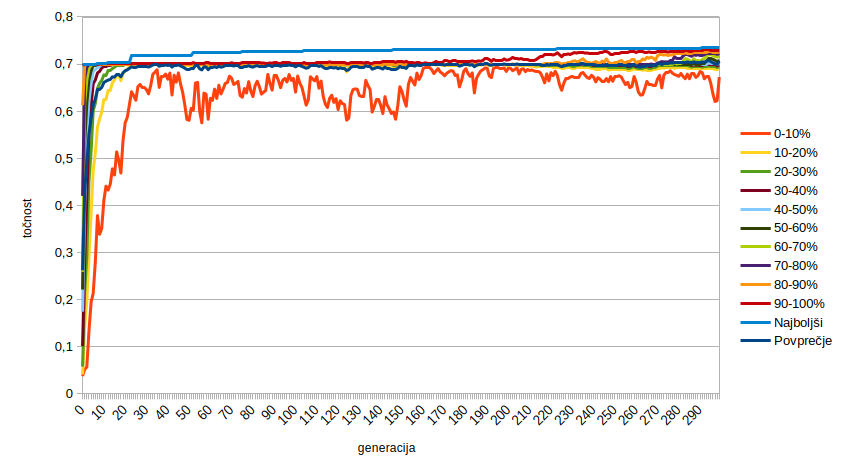
\includegraphics[width=13cm]{car/3/acc}
    \end{center}
    \caption{Graf točnosti populacije najboljšega agenta tretjega nabora skozi generacije.}
    \label{fig:car_acc_3}
\end{figure}

\begin{figure}[H]
    \begin{center}
        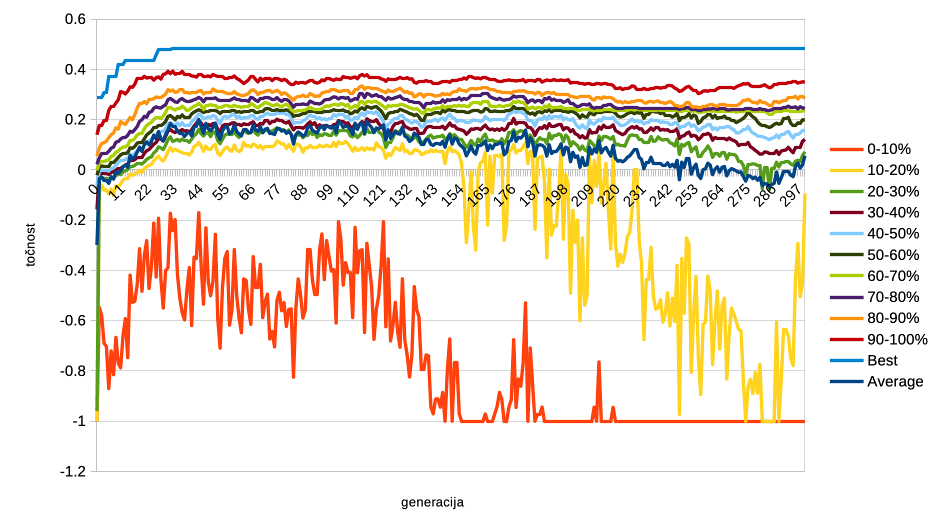
\includegraphics[width=13cm]{car/3/mcc}
    \end{center}
    \caption{Graf MCC populacije najboljšega agenta tretjega nabora skozi generacije.}
    \label{fig:car_mcc_3}
\end{figure}

\begin{figure}[H]
    \begin{center}
        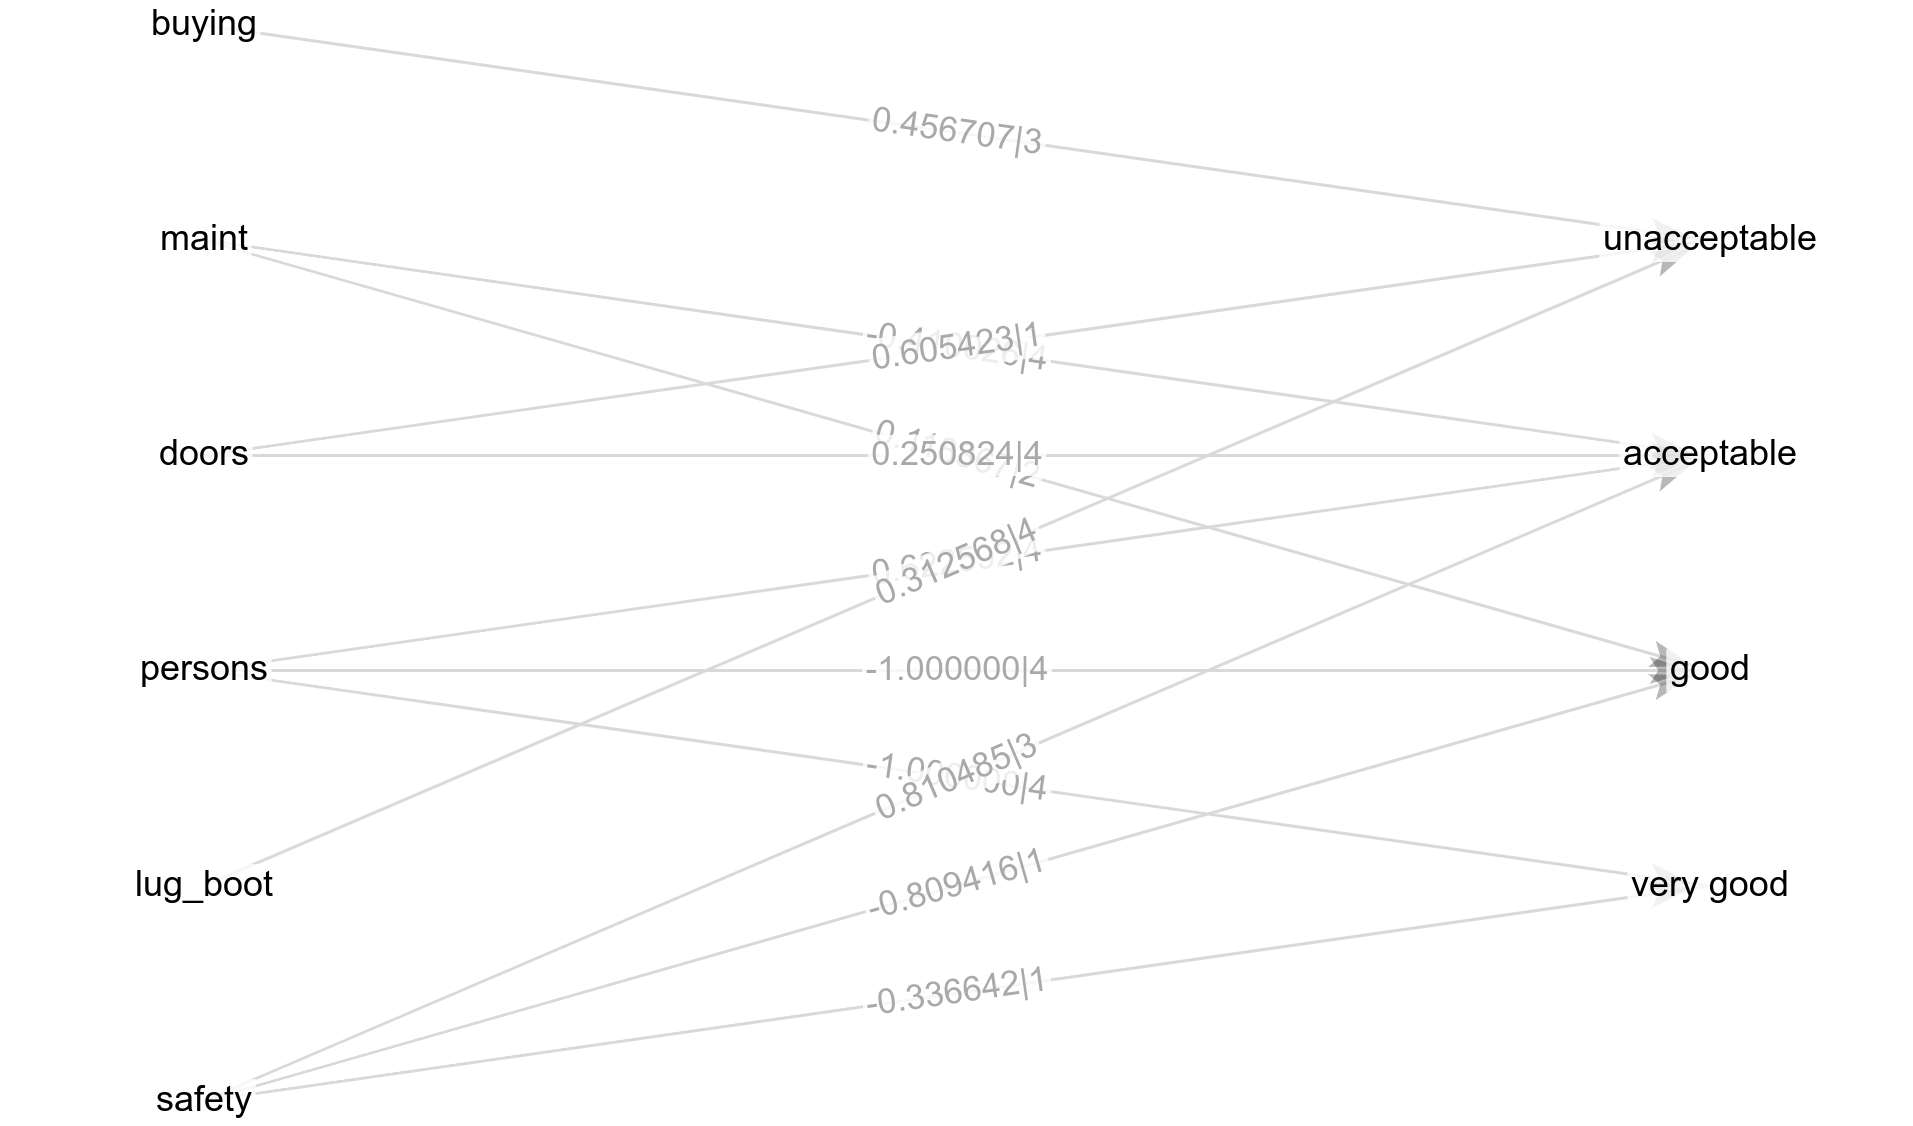
\includegraphics[width=13cm]{car/3/acc_g}
    \end{center}
    \caption{Vizualizacija najbolj točnega agenta tretjega nabora. Vsebuje 1 globoko vozlišče in 14 povezav.}
    \label{fig:car_acc_3_g}
\end{figure}

\begin{figure}[H]
    \begin{center}
        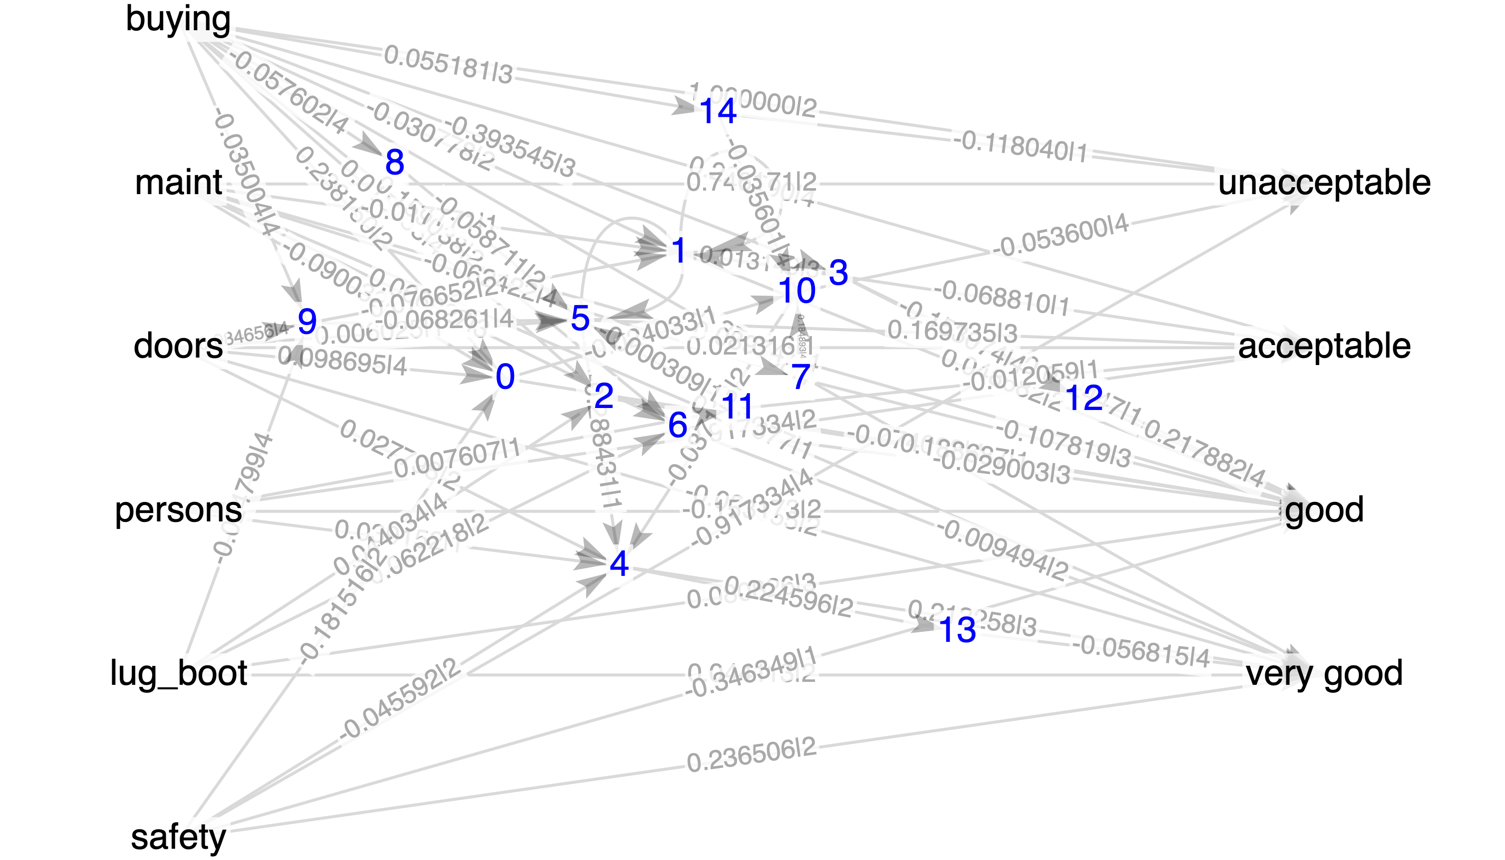
\includegraphics[width=13cm]{car/3/mcc_g}
    \end{center}
    \caption{Vizualizacija agenta z največjim MCC drugega nabora. Vsebuje 15 povezav.}
    \label{fig:car_mcc_3_g}
\end{figure}